\chapter{Wymagania funkcjonalne}
\label{Chapter3}

\section{Wstęp -- diagram przypadków użycia}

\begin{figure}[th]
\centering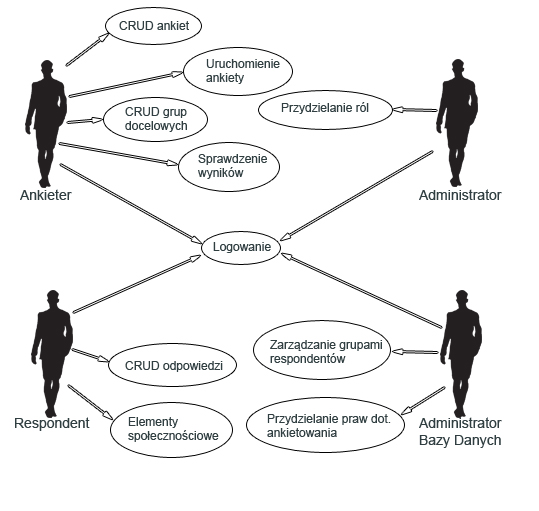
\includegraphics[width=15cm]{figures/UseCaseView}
\caption{Diagram przypadków użycia}\label{rys:usecase}
\end{figure}

Na rysunku 3.1 przedstawiono diagram przypadków użycia. W ramach Systemu udostępniane są różne funkcje, możliwe do wykonania przez różnych aktorów. Dla przykładu, Ankieter może tworzyć Badania i analizować ich Statystyki oraz Raporty, podczas gdy Respondent może odpowiadać w Ankietach w ramach skierowanych do niego Badań; Administrator zarządza przydzielaniem ról; Administrator Bazy Danych zajmuje zarządza grupami Respondentów i przydzielaniem praw i zezwoleń.

\section{Ankieter}

Poniżej przedstawiono przypadki użycia dotyczące Ankietera.

\subsection{UC01: Stworzenie Ankiety}

\ucsection{UC01: Stworzenie Ankiety}{Ankieter}
{Ankieter jest zalogowany w Systemie i chce utworzyć Ankietę}
{}{\ucactions{
\ucaction{1. Ankieter wpisuje atrybuty Ankiety: nazwę Ankiety, wstęp, podsumowanie}
\ucaction{2. System prezentuje stronę umożliwiającą dodawanie pytań}
\ucaction{3. Ankieter wybiera typ pytania}
\ucaction{4. Ankieter wpisuje treść pytania}
\ucaction{5. Ankieter podaje możliwe odpowiedzi}
\ucaction{6. System prezentuje podsumowanie ankiety}
\ucaction{7. Ankieter akceptuje ankietę}
\ucaction{8. System zapisuje ankietę w Katalogu Ankiet Ankietera}
}}
{\ucextensions{
\ucaction{4.A Typ pytania: pytanie otwarte}
\ucaction{4.A.1 Ankieter pomija krok 5.}
\ucaction{5.A Ankieter chce dodać kolejne pytanie}
\ucaction{5.A.1 Powrót do kroku 3.}
}}
{}

\subsection{UC02: Edycja Ankiety}

\ucsection{UC02: Edycja Ankiety}{Ankieter}
{
1. Ankieta znajduje się w Systemie i jest dostępna dla Ankietera \\
2. Ankieta nie jest częścią czynnego Badania \\
3. Ankieter jest zalogowany w Systemie i chce zmodyfikować istniejącą Ankietę
}
{}{\ucactions{
\ucaction{1. Ankieter wybiera Ankietę do modyfikacji}
\ucaction{2. System prezentuje wskazaną Ankietę}
\ucaction{3. Ankieter wybiera pytanie do edycji/usunięcia}
\ucaction{4. System prezentuje pytanie z możliwością edycji}
\ucaction{5. Ankieter edytuje/usuwa pytanie}
\ucaction{6. Ankieter potwierdza chęć zapisu zmienionej Ankiety}
\ucaction{7. System zapisuje zmienioną Ankietę}
}}
{\ucextensions{
\ucaction{5.A. Edycja możliwych odpowiedzi do pytań}
\ucaction{5.A.1 Ankieter edytuje możliwe odpowiedzi do pytań}
}}
{}

\subsection{UC03: Wybór Grupy Docelowej}

\ucsection{UC03: Wybór Grupy Docelowej}{Ankieter, Administrator Bazy Danych}
{
1. Ankieta znajduje się w Systemie i jest dostępna dla Ankietera \\
2. Grupa Docelowa znajduje się w Systemie i jest dostępna dla Ankietera \\
3. Ankieter jest zalogowany w Systemie i chce wybrać Grupę Docelową
}
{}{\ucactions{
\ucaction{1. Ankieter wybiera przycisk ,,Utwórz badanie''}
\ucaction{2. System prezentuje listę Grup Docelowych, do których Ankieter ma uprawnienia}
\ucaction{3. Ankieter wybiera Grupy Docelowe dla danej Ankiety}
\ucaction{4. Ankieter wybiera typ powiadamiania Respondentów}
\ucaction{5. Ankieter akceptuje powiązanie Grup Docelowych z Ankietą}
}}
{\ucextensions{
\ucaction{3.A. Zawężenie Grupy Docelowej}
\ucaction{3.A.1 Ankieter wybiera członków Grupy Docelowej, do której ma być skierowana Ankieta.}
\ucaction{3.A.2 Powrót do kroku 4.}
\ucaction{3.B. Grupa Docelowa poszukiwana przez Ankietera nie istnieje}
\ucaction{3.B.1 Ankieter próbuje połączyć kilka Grup Docelowych lub ich fragmentów}
\ucaction{3.B.2 W przypadku niepowodzenia kroku rozszerzenia 3.B.1, bądź wystąpienia takiej konieczności, Ankieter informuje Administratora Bazy Danych, że nie ma praw do wysyłania ankiet do wskazanych osób i/lub powiadamia go (za pomocą poczty elektronicznej) o potrzebie stworzenia Grupy Docelowej o konkretnych atrybutach (BC03)}
\ucaction{3.B.3 W przypadku pominięcia kroku rozszerzenia 3.B.2, powrót do kroku 4., w przeciwnym razie, powrót do kroku 1.}
}}
{}

\subsection{UC04: Uruchomienie Badania}

\ucsection{UC04: Uruchomienie Badania}{Ankieter, Respondent}
{
1. Ankieta znajduje się w Systemie i jest dostępna dla Ankietera \\
2. Ankieta jest powiązana z Grupą Docelową \\
3. Ankieter jest zalogowany w Systemie i chce rozesłać istniejącą Ankietę
}
{Respondenci powiadomieni o Ankiecie}{\ucactions{
\ucaction{1. Ankieter ustawia czas rozpoczęcia i zakończenia Ankiety}
\ucaction{2. Ankieter potwierdza chęć uruchomienia Badania}
\ucaction{3. System rozsyła Ankietę do Respondentów}
\ucaction{4. System powiadamia Respondentów o Ankiecie}
}}
{\ucextensions{
\ucaction{1.A. Ankieter chce prowadzić ankietę wielokrotną}
\ucaction{1.A.1 Ankieter ustawia częstotliwość ankiety}
}}
{}

\subsection{UC06: Sprawdzenie wyników}

\ucsection{UC06: Sprawdzenie wyników}{Ankieter}
{
1. Ankieta znajduje się w Systemie, zawiera odpowiedzi od Grupy Docelowej i jest dostępna dla Ankietera \\
2. Ankieter jest zalogowany w Systemie i chce pozyskać informacje od Studentów/Absolwentów
}
{Wygenerowany Raport}{\ucactions{
\ucaction{1. Ankieter wybiera Ankietę, której wyniki chce poznać}
\ucaction{2. Ankieter wybiera typ Raportu, który chciałby zobaczyć}
\ucaction{3. System generuje i wyświetla Raport}
}}
{}

\section{Respondent}

Poniżej przedstawiono przypadki użycia dotyczące Respondenta.

\subsection{UC05: Udzielenie odpowiedzi}

\ucsection{UC05: Udzielenie odpowiedzi}{Respondent}
{
1. Respondent dostaje powiadomienie o Ankiecie (link bezpośredni do Ankiety) \\
2. Respondent jest zalogowany w Systemie i chce wypełnić Ankietę
}
{}{\ucactions{
\ucaction{1. System prezentuje Ankietę Respondentowi}
\ucaction{2. Respondent udziela odpowiedzi na pytania}
\ucaction{3. System prezentuje podsumowanie odpowiedzi}
\ucaction{4. Respondent zatwierdza wypełnioną Ankietę}
\ucaction{5. System zapisuje odpowiedzi}
}}
{\ucextensions{
\ucaction{1.A. Przedawniona Ankieta}
\ucaction{1.A.1 System informuje, że Ankieta już się zakończyła}
\ucaction{5.A. Brak odpowiedzi na niektóre pytania}
\ucaction{5.A.1 System informuje, że pozostały pytania bez odpowiedzi}
\ucaction{5.A.2 Powrót do kroku 2.}
}}
{}

\section{Administrator Bazy Danych}

Poniżej przedstawiono przypadki użycia dotyczące Administratora Bazy Danych.

\subsection{UC07: Tworzenie Grupy Docelowej}

\ucsection{UC07: Tworzenie Grupy Docelowej}{Administrator Bazy Danych}
{
1. Ankieter chce wysyłać Ankiety do określonych Respondentów w prosty sposób \\
2. Administrator Bazy Danych jest zalogowany w Systemie i chce utworzyć nową Grupę Docelową
}
{Nowa Grupa Docelowa w Systemie}{\ucactions{
\ucaction{1. Administrator Bazy Danych wybiera opcję tworzenia Grup Docelowych}
\ucaction{2. System prezentuje formularz tworzenia Grupy Docelowej}
\ucaction{3. Administrator Bazy Danych wprowadza nazwę tworzonej Grupy Docelowej, wybiera Grupę Nadrzędną oraz Respondentów do dodania do Grupy Docelowej}
\ucaction{4. Administrator Bazy Danych potwierdza chęć stworzenia Grupy Docelowej}
\ucaction{5. System zapisuje nową Grupę Docelową}
}}
{\ucextensions{
\ucaction{4.A Brak Grupy Nadrzędnej}
\ucaction{4.A.1 Administrator Bazy Danych nie uzupełnia Grupy Nadrzędnej}
}}
{}

\subsection{UC08: Edycja Grupy Docelowej}

\ucsection{UC08: Edycja Grupy Docelowej}{Administrator Bazy Danych}
{
1. Grupa Docelowa znajduje się w Systemie \\
2. Administrator Bazy Danych jest zalogowany w Systemie i chce zmodyfikować Grupę Docelową
}
{Zmodyfikowana lista członków Grupy Docelowej}{\ucactions{
\ucaction{1. Administrator Bazy Danych wybiera Grupę Docelową}
\ucaction{2. Administrator Bazy Danych wybiera członka\slash członków Grupy Docelowej do edycji\slash usunięcia}
\ucaction{3. Administrator Bazy Danych dodaje\slash edytuje]\slash usuwa członka\slash członków Grupy Docelowej}
\ucaction{4. Administrator Bazy Danych potwierdza chęć wprowadzenia zmian}
\ucaction{5. System zapisuje zmiany}
}}
{}

\section{Wszyscy Użytkownicy}

Poniżej przedstawiono przypadki użycia dotyczące wszystkich Użytkowników.

\subsection{UC09: Logowanie do Systemu}

\ucsection{UC09: Logowanie do Systemu}{Użytkownik (Ankieter, Administrator, Administrator Bazy Danych, Respondent)}
{Użytkownik posiada konto w Systemie i posiada poprawne dane logowania}
{Użytkownik jest zalogowany w Systemie}{\ucactions{
\ucaction{1. System wyświetla Użytkownikowi formularz logowania}
\ucaction{2. Użytkownik podaje login lub adres e-mail oraz hasło}
\ucaction{3. System uwierzytelnia Użytkownika}
}}
{\ucextensions{
\ucaction{2.A Użytkownik chce się zalogować przy pomocy eKonta}
\ucaction{2.A.1 Użytkownik wybiera opcję logowania przez eKonto}
\ucaction{2.A.2 System przekierowuje Użytkownika na stronę logowania przez eKonto (eLogin)}
\ucaction{2.A.3 Użytkownik wprowadza dane logowania do eKonta}
\ucaction{2.A.4 Powrót do kroku 3.}
}}
{}